Due to the large Monte Carlo modeling uncertainties of the top background with
large $\met$, in the analysis with the 2015 data this process had one of the
largest uncertainties. For this reason, in order to increase the precision of
the analysis with the combined 2015 and 2016 data, the Top control region
($\crtop$) is used to estimate the contribution of $t \bar{t}$ and single top
processes in the signal region. In addition to cuts from A to H as defined in
\cref{sec:event-selection-1} the $\crtop$ region selects events with:
\begin{itemize}
\item Events containing an electron are vetoed.
\item Exactly one good muon.
\item The transverse mass defined in \eqref{eq:99} satisfies
  $30 < m_\mathrm{\, T} < 100$~GeV.
\item At least one of the selected jets in the event is identified as a $b$-jet.
\end{itemize}
\cref{fig:top_plots} report the $\met$ and the leading jet $\pt$ distributions
after the background only fit described in
\cref{sec:glob-simult-likel,sec:fit-strategy}. It shows, within uncertainties, a
good agreement between data and \gls{mc}.
\begin{figure}[!th]
  \centering
  \begin{subfigure}[t]{.48\linewidth}
    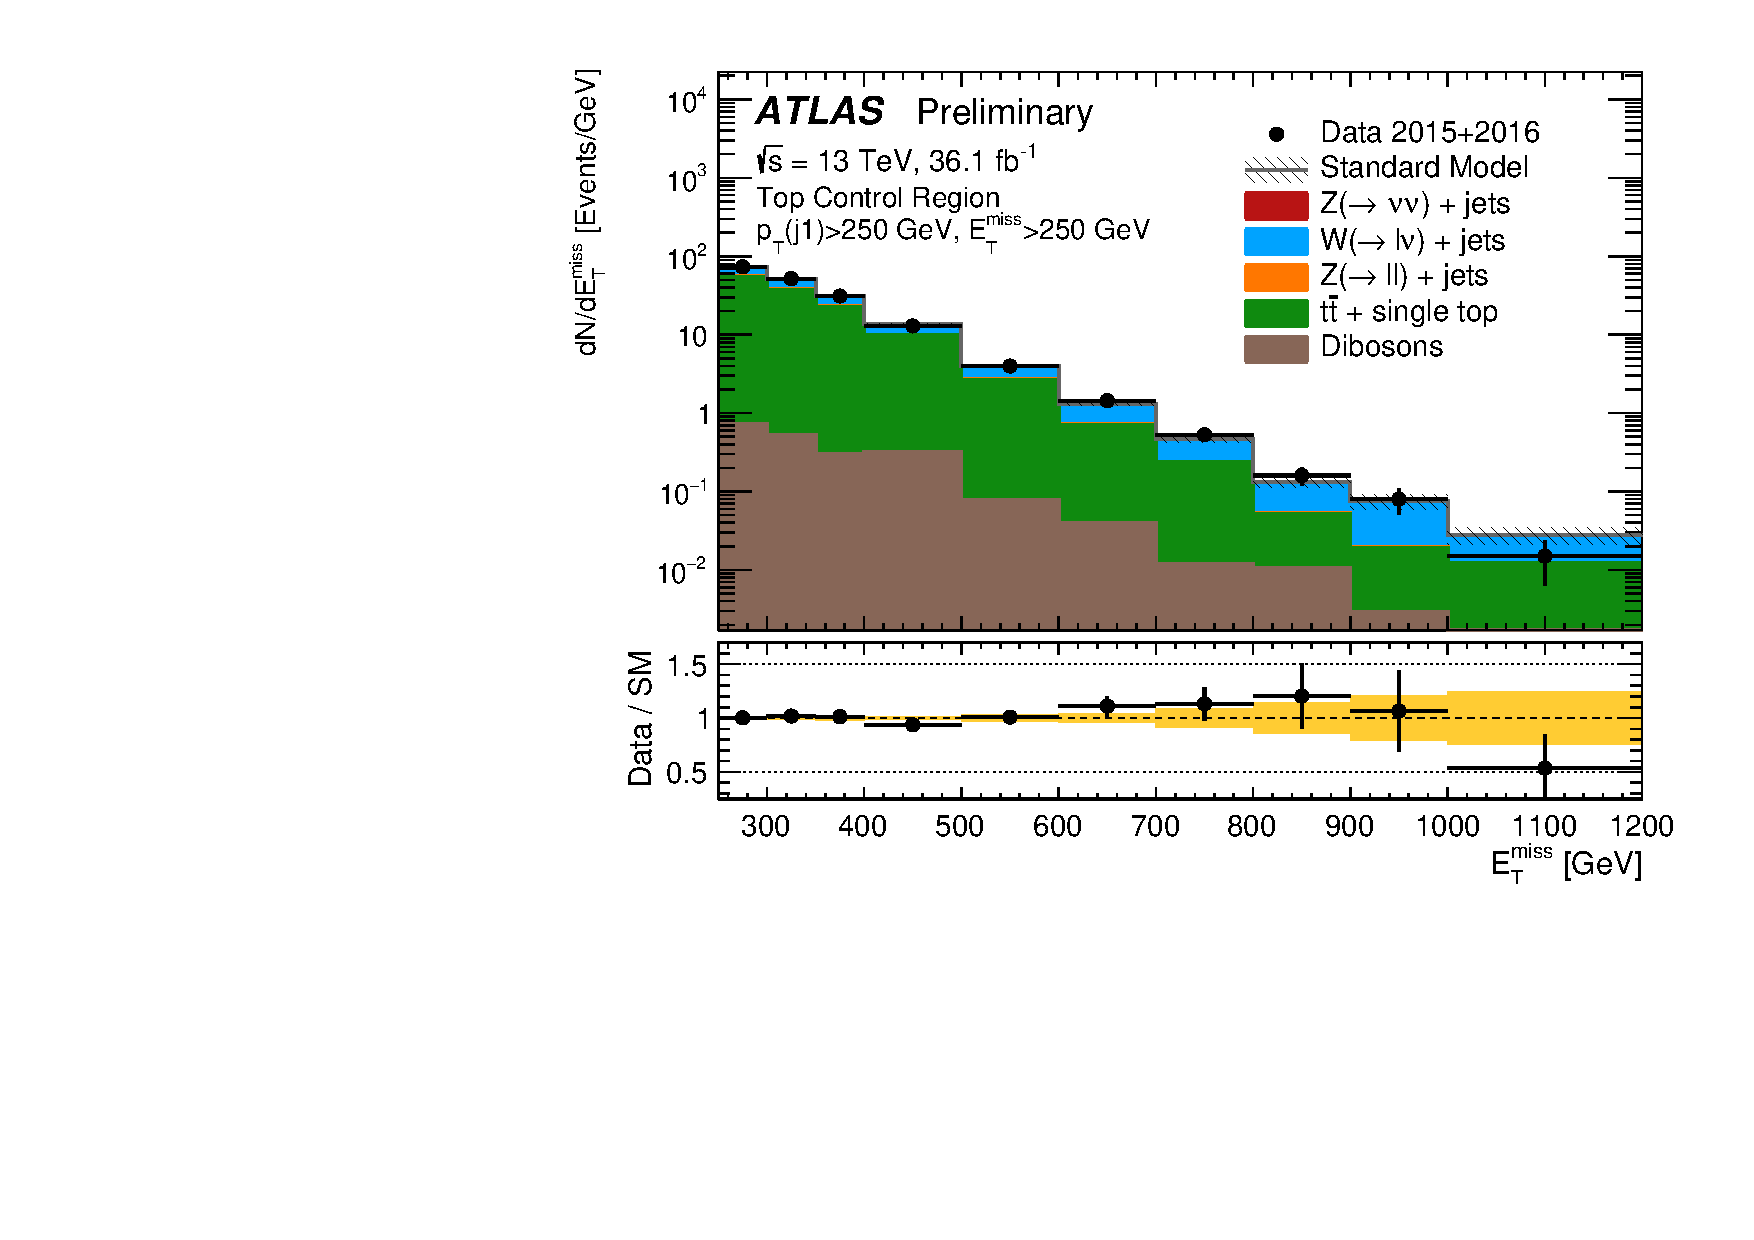
\includegraphics[width=\linewidth]{top_cr_met}
    \caption{$\met$ distribution.}
    \label{fig:top_cr_et_miss}
  \end{subfigure}
  \begin{subfigure}[t]{.48\linewidth}
    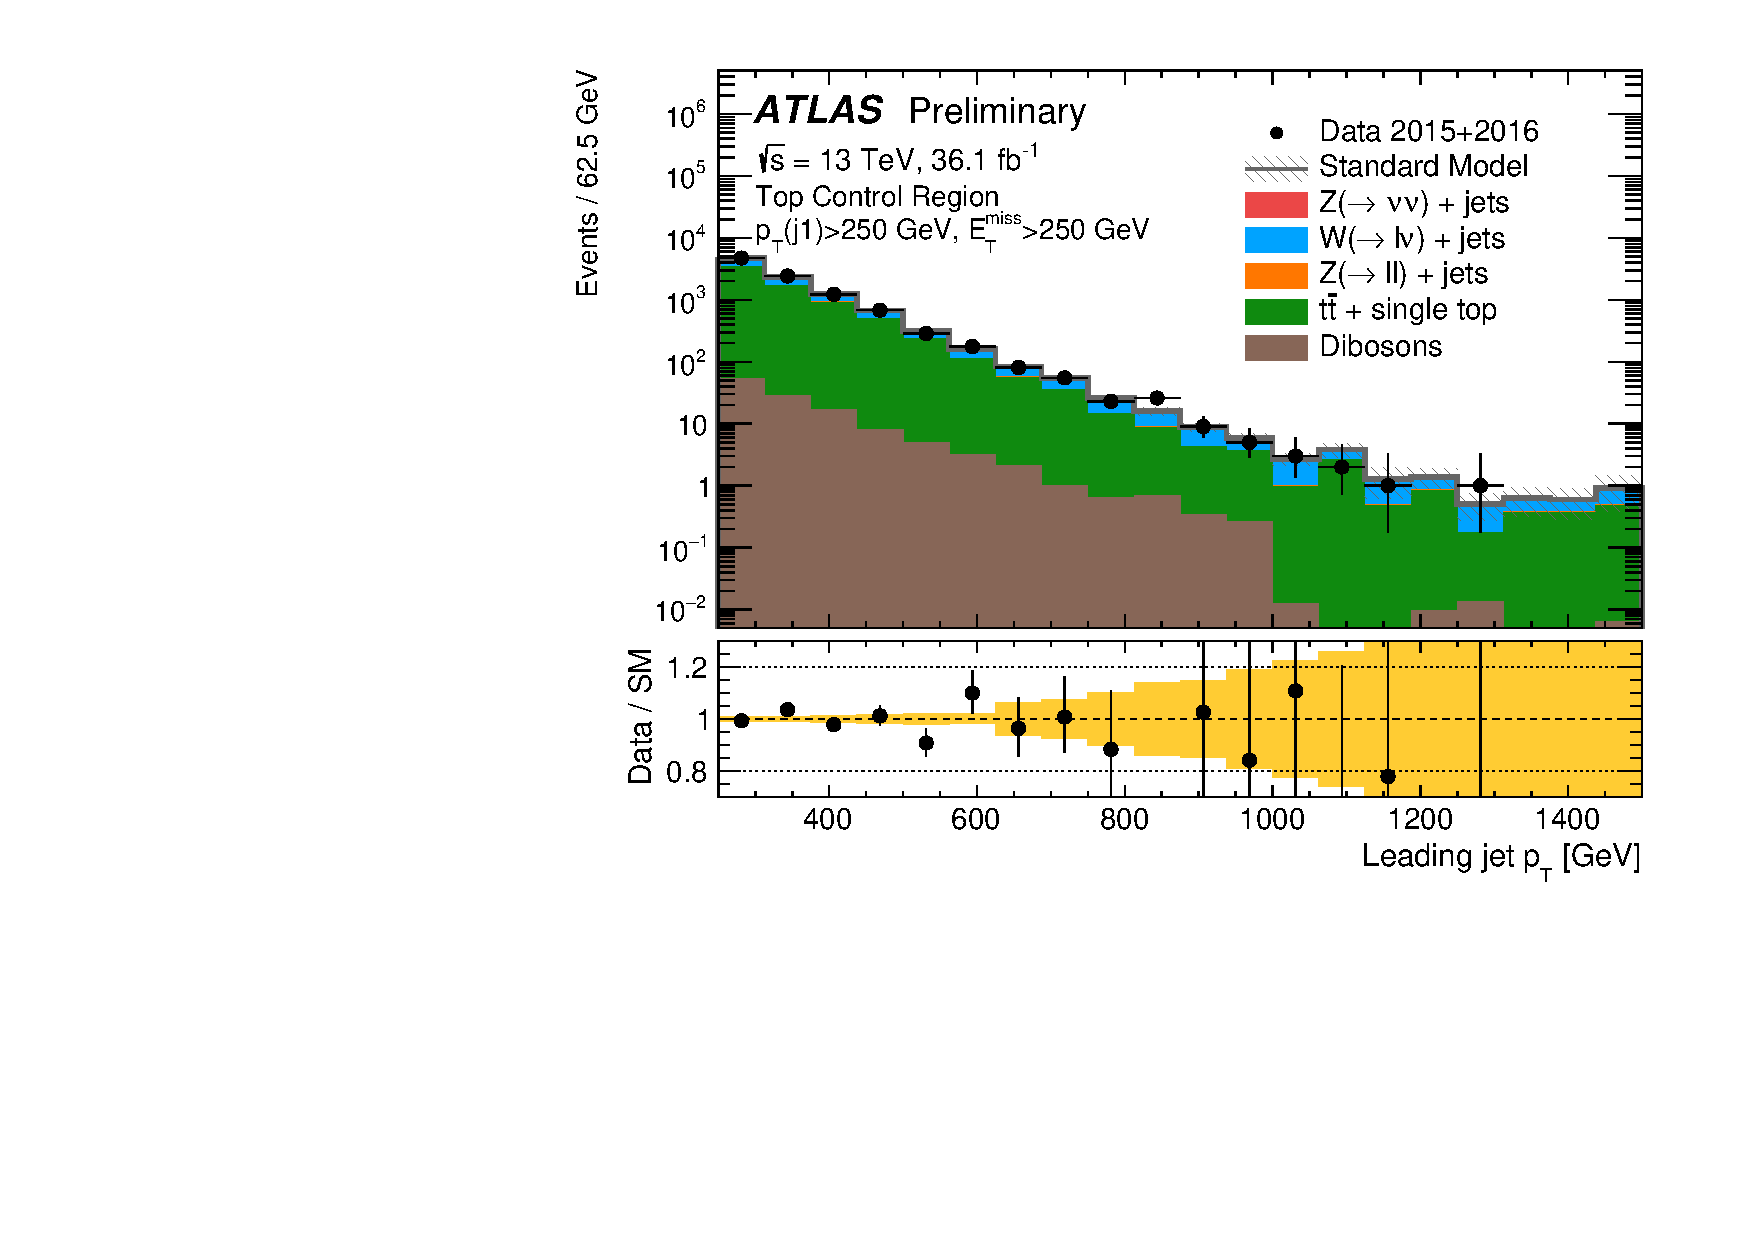
\includegraphics[width=\linewidth]{top_cr_jet1}
    \caption{Leading jet $\pt$ distribution.}
    \label{fig:top_cr_jet1}
  \end{subfigure}
  \caption{Observed and predicted $\met$ and leading jet $\pt$ after the
    background only fit in the $\crtop$ control region for the $\met > 250$~GeV
    inclusive selection. The error bands in the ratio plot on the bottom of the
    figures include statistical and systematic uncertainties. The negligible
    contribution of \gls{ncb} and diboson backgrounds is not reported in the
    figure.}
  \label{fig:top_plots}
\end{figure}
%%% Local Variables:
%%% mode: latex
%%% TeX-master: "../search_for_DM_LED_with_ATLAS"
%%% End:
